\documentclass[../main.tex]{subfiles}

\begin{document}
    \chapter{Introduction}\label{chap:intro}

    After many decades of ups and downs, deep learning techniques recently produced unprecedented breakthroughs
    in complex domains like computer vision, speech recognition, and natual language processing. \\
    Deep learning~\cite{deeplearning} is a subset of machine learning based on Artificial Neural Networks---statistical models loosely
    inspired by insights from neuroscience. \\
    Two were the main enablers for this revolution: the ever increasing availability of large labeled
    datasets and the terrific growth of computational power that took place in recent years, in particular
    the advent of GPUs to speed-up by orders of magnitude the kind of computations needed by deep learning.

    \begin{figure}[h!]
        \centering{}
        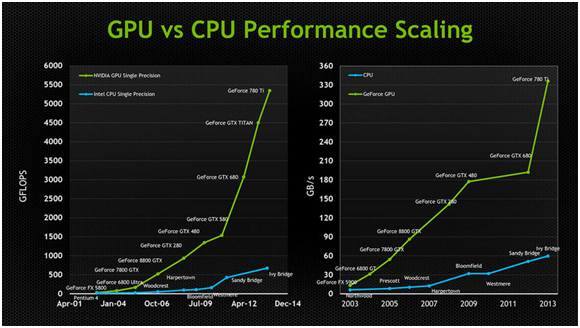
\includegraphics[width=300px]{img/gpu-vs-cpu.png}
        \caption{GPUs are optimized for parallel tasks, and thus are particularly suited to carry out computations
        like matrix multiplication, which is obiquitous in deep learning.}\label{fig:gpu-vs-cpu}
    \end{figure}

    In computer vision in particular, state-of-the-art approaches for tasks such as image recognition,
    object detection and image segmentation all have Convolutional Neural Networks (CNNs)~\cite{lecun-89e} at their core,
	a specialization of the more general feedforward network architecture to deal with data with a grid-like topology,
    like images.

    Like the majority of machine learning technologies, also deep learning relies on the i.i.d.\ assumptions,
    a set of assumptions drawn from statistical learning theory~\cite{Vapnik1998} by which the training and the test sets are generated
    from the same data generating process, i.e.\ they came from the same distribution. \\
    Neural Networks are known for their great generalization capabilities. In fact, when trained on very large
    datasets, such as ImageNet~\cite{imagenet}, CNNs can be used to extract meaningful features from new datasets, on top of which
    a linear classifier (e.g. Linear SVM or Logistic Regression) can be successfully trained.
    This method goes under the name of Transfer Learning~\cite{transfer-learning}. \\

    Transfer learning works well when the training and test sets came from very similar distributions. When this condition
    is not met, CNNs tends to perform poorly despite their outstanding generalization capabilities.
    Hence, techniques are needed to deal with such cases. \\
	The problem of dealing with settings in which the i.i.d.\ assumptions
	do not hold is known as Domain Adaptation~\cite{domain-adaptation-review}, in which we seek to minimize generalization error
	in those situations in which there is a distribution shift between the training set
	(called source domain in domain adaptation terminology) and the test set (target domain). \\
    A satisfying solution to this problem would be very appealing, because it would mean being able to train offline huge
	models on very large datasets,
    and having them generalize well when deployed on a real-world scenario. Imagine for instance a mobile app in which users can
    take photos, which should be analyzed (e.g.\ classified) by the app in some way. These photos are likely to come from a different
    distribution from that of ImageNet. Having a model perform well on this target domain from the first use can represent an
	advantage from a user experience perspective. \\

    This work is about designing techniques to deal with situations in which plain transfer learning does not work well.
	In particular, we focused on those cases where the domain shift is caused by object transformations, such as
    translation and scale. This is because we are mainly interested in robotics applications, in which a robot
    might take pictures from very different angles and viewpoints---a situation which is very different from that of
    the majority of image recognition datasets, in which the object always appears at the center of the image. \\

    The rest of the thesis is organized as follows. After a review of background concepts on domain
    adaptation and deep learning in~\autoref{chap:background}, we review recent literature in~\autoref{chap:related}.
    In~\autoref{chap:approach} we describe our approach, the Domain Multiplicative Fusion (DMF) Network, describing
    the main components and the techniques it builds upon. In~\autoref{chap:experiments} and~\autoref{chap:comparison},
    experiments across a variety of robotics datasets and network architectures are reported.
    The thesis concludes with~\autoref{chap:summary} with a summary and a discussion on future research.

\end{document}
